\documentclass[12pt]{beamer}
\usepackage{breqn}
\usepackage[brazilian,hyperpageref]{backref}
\usepackage[num]{abntex2cite}		% Citações padrão ABNT
\usepackage[utf8]{inputenc}
\usepackage[portuguese]{babel}
\usepackage{colortbl}
\usepackage{color}
\usepackage{amsmath}
\usepackage{url}
\usepackage{hyperref}
\usepackage{beamerthemeshadow}
\usepackage{verbatim}
\usepackage{listings}

\graphicspath{{../images/}}
\citebrackets[]

\setbeamertemplate{bibliography item}{\insertbiblabel}
\setbeamertemplate{caption}[numbered]

\renewcommand{\backrefpagesname}{Citado na(s) página(s):~}
% Texto padrão antes do número das páginas
\renewcommand{\backref}{}
% Define os textos da citação
\renewcommand*{\backrefalt}[4]{}
    %\ifcase #1 %
        %Nenhuma citação no texto.%
    %\or
        %Citado na página #2.%
    %\else
        %Citado #1 vezes nas páginas #2.%
    %\fi}%

\beamertemplatenavigationsymbolsempty% tira os elementos de navegação da parte de baixo
%\setbeamertemplate{footline}{}%remove o autor e o título da parte de baixo

\addtobeamertemplate{navigation symbols}{}{%
    \usebeamerfont{footline}%
    \usebeamercolor[black]{footline}%
    \hspace{1em}%
    \insertframenumber/\inserttotalframenumber%
}

\usetheme{Frankfurt}
\usecolortheme{orchid}

\author[Victor * Almeida *]{Victor Emanuel Almeida \and Victor Hugo Almeida Alicino}
\title[Financiamento de veículos]{Financiamento de Veículos novos e seminovos para empresa Almeida Carros}
\subtitle{Sistema Especialista}
\date{\today}
\institute{UNIOESTE}
\logo{
\includegraphics[height=1cm]{logo_unioeste.jpg}}

\definecolor{dkgreen}{rgb}{0,0.6,0}
\definecolor{gray}{rgb}{0.5,0.5,0.5}
\definecolor{mauve}{rgb}{0.58,0,0.82}
\definecolor{laranja_claro}{rgb}{1,0.9,0.5}
\definecolor{laranja_escuro}{rgb}{1,0.5,0.2}
\definecolor{azul_claro}{rgb}{0.5,0.9,1}

\lstset{frame=tb,
    language=C++,
    frame=tb,
    aboveskip=3mm,
    belowskip=3mm,
    showstringspaces=false,
    columns=flexible,
    basicstyle={\small\ttfamily},
    numbers=left,
    numberstyle=\tiny\color{gray},
    keywordstyle=\color{blue},
    commentstyle=\color{dkgreen},
    stringstyle=\color{mauve},
    breaklines=true,
    breakatwhitespace=true,
    xleftmargin=.05\textwidth,
    xrightmargin=.05\textwidth,
    tabsize=4,
}

\begin{document}
\frame{\titlepage}

\begin{frame}
    \frametitle{Conteúdo}
    \tableofcontents
\end{frame}

\section{Contextualização}
\begin{frame}
    \frametitle{Proposta}

    \large Implementar sistema especialista para identificar a melhor financeira, dentro das parceiras da Almeida carros, para financiar carros novos e seminovos tendo como base o perfil do cliente e características do carro.

\end{frame}

\begin{frame}
    \frametitle{Definição Financiamento}
    \textbf{Financiamento}: ``é o ato de uma organização, usualmente uma empresa, que ajuda a pagar um produto ou um serviço de uma pessoa, ou de outra empresa, através de doação de dinheiro ou empréstimo''\cite{financiamento}.
\end{frame}

\begin{frame}
    \frametitle{Mercado}
    \begin{itemize}
        \item Em 2021 o mercado de carros seminovos cresceu 17.8\%, 15.1 milhões de carros foram vendidos no Brasil\cite{mercado_seminovos};
        \item Em 2021 teve redução no número de financiamentos 3.5 milhões de carros financiados\cite{financiamento_2022};
        \item Uma boa porção dos veículos vendidos são financiados.
    \end{itemize}
\end{frame}

\section{Especialista}
\begin{frame}
    \frametitle{Especialista}
    \begin{itemize}
        \item\textbf{Nome}: Solange Cristina de Siqueira Almeida;
        \item\textbf{Formação}: Bacharel em Administração pela UNIOESTE, pós-graduada em Marketing Digital pela UNICESUMAR\@;
        \item\textbf{Profissão}: Administradora da Almeida Carros \url{https://almeidacarros.com.br/} e correspondente bancária certificada pelo FEBRABAN\@;
        \item\textbf{E-mail}: \url{soll30@hotmail.com}.
    \end{itemize}
\end{frame}

\section{Entrevistas}
\begin{frame}
    \frametitle{Entrevistas realizadas}

    \begin{itemize}
        \item Dia 02 de janeiro de 2023: Primeira entrevista com o objetivo de descobrir condições específicas para cada financeiras;
        \item Dia 26 de março de 2023: Segunda entrevista com o objetivo de validar a árvore;
        \item TODO:
    \end{itemize}

\end{frame}

\section{Sistema}

\begin{frame}
    \frametitle{Árvore montada a partir da primeira entrevista I}
    \begin{figure}
        \centering
        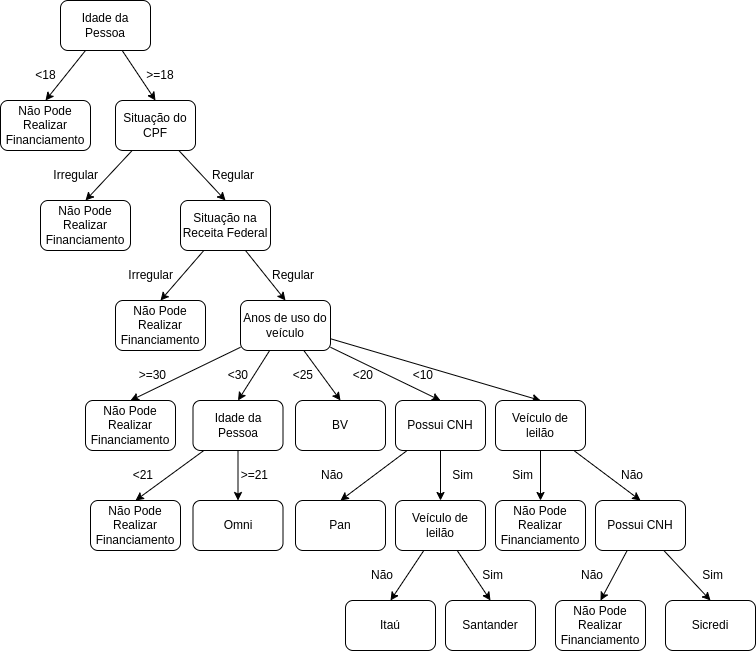
\includegraphics[height=.70\textheight]{1.png}
        \caption{Árvore completa}
    \end{figure} 
\end{frame}

\begin{frame}
    \frametitle{Árvore montada a partir da primeira entrevista II}
    \begin{figure}
        \centering
        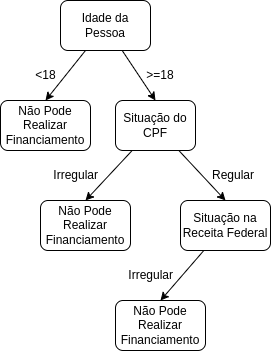
\includegraphics[height=.70\textheight]{condicoes_nao_aprova.png}
        \caption{Condições que impedem a concessão de crédito}
    \end{figure} 
\end{frame}

\begin{frame}
    \frametitle{Mão na massa!!}
    \begin{figure}
        \centering
        
\includegraphics[width=.3\textwidth]{pizza.png}
        
\includegraphics[width=.3\textwidth]{rolo.png}
        
\includegraphics[width=.3\textwidth]{burrito.png}
    \end{figure}
\end{frame}

\section{Considerações finais}
\begin{frame}[allowframebreaks]
    \frametitle{Referências}
    \bibliography{ref}
\end{frame}

\begin{frame}
    \frametitle{Contatos}
    \centering
    \url{victor.alicino@gmail.com}
    \url{archvictor@protonmail.com}
\end{frame}

\end{document}
